%! Licence = CC BY-NC-SA 4.0

%! Author = gianfluetsch, mariuszindel, marcomartinez
%! Date = 30. Dez 2021
%! Project = cydef_summary

\section{Velociraptor}
Use Velociraptor to collect evidence, hunt for IOCs or just to monitor for something to happen. For that purpose, there are different kinds of client and server artifacts (scripts to collect stuff) some general and some that trigger on events which you could use for
monitoring.\\

Velociraptor is a free and open-source software project developed by the Velocidex Company. Velociraptor is generally based on GRR, OSQuery, and Google's Rekall tools. Velociraptor allows users to collect Forensics Evidence, Threat Hunting, Monitoring artifacts, Executing remote triage process. As an open-source platform, Velociraptor continues to improve and evolve through inputs and feedback of digital forensics investigation and cybersecurity practitioner

Velociraptor was released in 2019 and allows for hunting across many thousands of machines. Inspired by OSQuery, Velociraptor implements a new query language dubbed \textit{VQL} (Velociraptor Query Language) which is similar to SQL but extends the query language in a more powerful way. Velociraptor also emphasizes ease of installation and very low latency - typically collecting artifacts from thousands of endpoints in a matter of seconds.

\subsection{Introduction}

\subsubsection{Terminology}
\begin{itemize}
    \item \textbf{File}
    \begin{itemize}
        \item  File system access based on OS FS API
    \end{itemize}
    \item \textbf{NTFS}
    \begin{itemize}
        \item NTFS raw parsing filesystem access
    \end{itemize}
    \item \textbf{Registry}
    \begin{itemize}
        \item Windows Registry access using the Registry API
    \end{itemize}
    \item \textbf{Artifacts}
    \begin{itemize}
        \item Artifacts collected from the client incl. type and time in Velociraptor Artifacts are commands and scripts that actually grab some data (we usually call these artifacts) from clients. Structured in YAML
    \end{itemize}
    \item \textbf{VQL}
    \begin{itemize}
        \item Velociraptor Query Language
    \end{itemize}
    \item \textbf{Hunting}
    \begin{itemize}
        \item enables you to collect the same artifacts over an entire fleet
    \end{itemize}
\end{itemize}

\subsubsection{Virtual File System (VFS)}
\begin{itemize}
    \item File - File system access based on OS FS API
    \item NTFS - NTFS raw parsing filesystem access
    \item Registry - Windows Registry access using the Registry API
    \item Artifacts - Artifacts collected from the client incl. type and time
    in Velociraptor Artifacts are commands and scripts that actually
    grab some data (we usually call these artifacts) from clients.
\end{itemize}

\columnbreak

\subsubsection{Velociraptor Hunts}
Hunting enables you to collect the same artifacts over an entire fleet. For example execute a powershell script and collect stdout.

\begin{itemize}
    \item Only systems that are connected will participate in the hunt
    \item Only systems that are connected will deliver results
    \item Hunts are run for quite some time (days), repeatedly
    \item Hunts may be restricted by label or OS
\end{itemize}
\textbf{Warning:} Disk Space, Clientperformance and Networkload can negativly impact infrastructure.

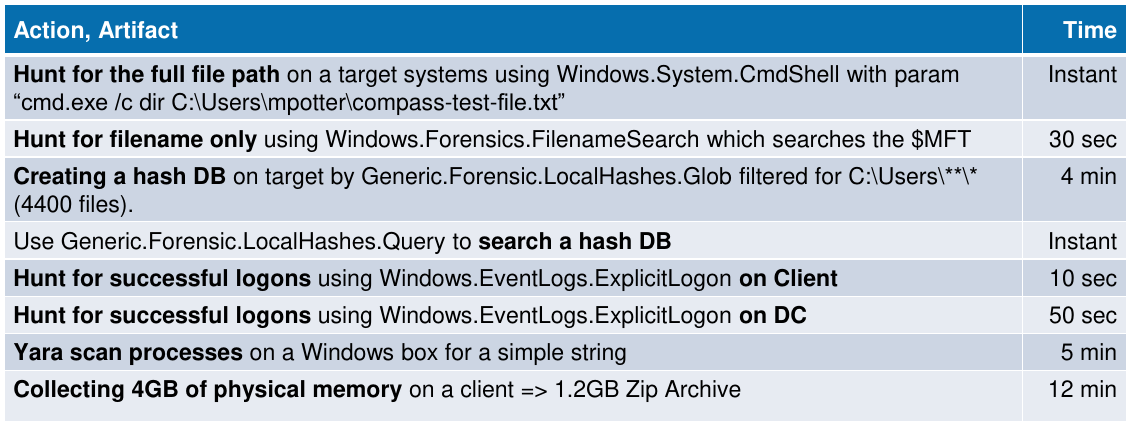
\includegraphics[width=\linewidth]{./img/10-velociraptor/velo_speed}

\subsubsection{Velociraptor Notebooks}
Can have text with a VQL query.

\subsubsection{Velociraptor Query Language}
What is VQL:
\begin{itemize}
    \item It looks like SQL
    \item Everything in Velociraptor is basically returning Table (Resultset)
    \item Functions and plugins are the major accelerators
\end{itemize}
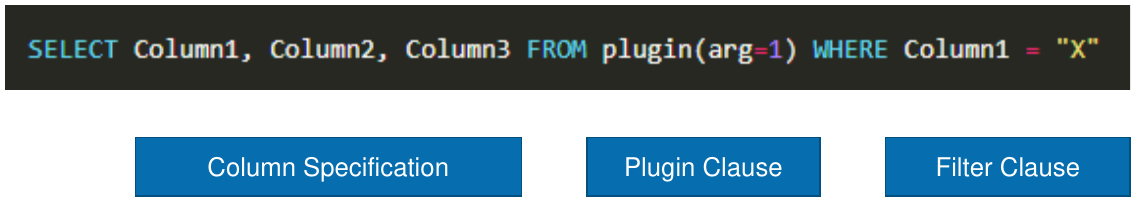
\includegraphics[width=\linewidth]{./img/10-velociraptor/vql.png}

\begin{lstlisting}
-- comment
// comment

#If you want to match strings
SELECT * FROM pslist() WHERE Exe =~ "veloci"

#Put values or entire queries into a variable using LET
LET test = "gugus"
LET test = SELECT * FROM pslist()

#using LIMIT
SELECT * FROM glob(globs="C:/**") LIMIT 5

#Use log() to do Candle-Light Debugging
SELECT Null FROM pslist() WHERE log(message="yeah, hit line")

#Use the glob plugin to get a list of files easily.
SELECT Name FROM glob(globs= "C:/Users/**/Downloads/*.ex?") LIMIT 5

Globs support wildcards such as
? for a single letter
* part of a string
** used to traverse recursively into folder

#Globs support different file accessors e.g. the Registry
SELECT FullPath, Name, Data.type, Data.value FROM glob(globs= "HKEY_USERS/*/Software/**/*", accessor="reg")

#Use if to branch depending on a condition
SELECT * FROM if(
    condition=Exe =~ "chrome",
    then={ expression or query },
    else={ expression or query }
    // else is optional
)

#You may loop over result sets using foreach applying a sub query
LET foo = SELECT * FROM pslist() where Exe =~ "chrome" LIMIT 5
SELECT * FROM foreach(
    row=foo,
    query={SELECT * FROM handles(pid=Pid)}
)

#Create a query that lists loaded DLLs for Velociraptor including compile time and signature
LET pids = SELECT * FROM pslist() WHERE Exe =~ "veloci"
SELECT * FROM foreach( row = pids, query = {
    SELECT Pid, ExePath, parse_pe(file=ExePath) .FileHeader.TimeDateStamp as
    CompileTime, authenticode(filename=ExePath) .SubjectName as Subject,
    authenticode(filename=ExePath) .Trusted as Trusted FROM modules(pid=Pid)
})
\end{lstlisting}

\subsubsection{Registry Search}
Velociraptor can be used to search the registry of a client in several ways
\begin{enumerate}
    \item Manually look through the registry
    \item Design your own VQL query and use the Notebook
    \item Run a hunt on only Forensic to get the information
\end{enumerate}

\subsubsection{Notebook - raw\_reg}
Like the \textit{raw\_reg} accessor, the zip accessor also requires a url. Here is what a query for all files ending with .jpg in the zip file \lstinline|C:\Users\Bob\Desktop\images.zip| could look like:

\begin{lstlisting}[language=bash]
    SELECT * FROM glob(globs=url(scheme='ntfs', path ='C:/Users/Bob/Desktop/images.zip', fragment='/**/*.jpg').String, accessor='zip')
\end{lstlisting}

\subsubsection{Notebook - foreach}
To not only do this for the current user but all users, you have to use a \textit{foreach} plugin.

The following statement would give you the Name and executable path for all executables that are running as the user(s) with the SID that is also running a process that has velociraptor in its executable path.

\begin{lstlisting}[language=bash]
    SELECT * FROM foreach(
    row={SELECT OwnerSid AS velociraptor_owner FROM pslist() WHERE Exe=~'velociraptor'},
    query={SELECT Name, Exe FROM pslist() WHERE OwnerSid=velociraptor_owner}
)
\end{lstlisting}

\subsubsection{Builtin Artifacts}
Velociraptor already comes with a number of pre-built artifacts for frequently needed queries.
This includes for example querying the registry (\lstinline|Windows.Registry.NTUser|).

\subsubsection{YARA Artifact}
You might have to use a foreach loop again where the rows statement gives you the PIDs and names of all processes and then scan for the YARA signature in the query block.



\subsection{Lateral Movement}
Lateral movement means to move within the internal network to access the organization's target data and to exfiltrate the data. In this challenge you will solve tasks to detect lateral movement using Velociraptor.

\subsubsection{Detection PsExec}
To Detect if someone used \textit{PsExec} after passing the hash, there are multiple ways. One way is to design your own Artifact based on \lstinline|Windows.Registry.Sysinternals.Eulacheck| Artifact.

\subsubsection{Use Velociraptor Artifact}
In Velociraptor, use the Artifact \lstinline|Windows.EventLogs.AlternateLogon|. It will list all Windows events with ID \textit{4648}. Use the timestamp function from Velociraptor to change the timestamp to date time format.

\subsubsection{Event Correlation}
With the event results from the Artifacts used, do an event correlation by matching the time at which both events occurred. Both event should have a temporal correlation.

\subsubsection{Evidence on Destination}
As you will see in the result of Artifact \lstinline|Windows.EventLogs.AlternateLogon|, the TargetServerName was DC1. Look for evidence of execution on destination DC1 by searching for event ID \textit{4624} as mentioned in SANS Hunt Evil Poster.

\subsubsection{Detection Mimikatz}
Now you have collected some evidence that someone did misuse \textit{PsExec} for passing the hash. But to dump the hash from a node, you need a tool. One such tool is Mimikatz. Use the \lstinline|Windows.System.Amcache| Artifact to detect if Mimikatz was executed on the system.